\chapter{Experimentation}

In this chapter multiple graphs are depicted.
These graphs are generated by reading every database of every node.
The blocks are depicted as nodes and the previous hash pointers are edges in the graph.
The nodes have added colouring to indicate extra meaning.
Green nodes are a first block in a MultiChain of a peer,
and as such have no inbound arrows.
Blue nodes are a sequential block between the same previous peers,
therefore they do not have two inbound arrows.
Red nodes are half-signed blocks,
and therefore only have one inbound and one outbound arrow.

\section{Software engineering tests}
MultiChain is tested in several ways to verify it is correctly working
following standard software engineering practices.
The enforcement of these types of tests is a policy recently introduced within Tribler.

\subsection{Unit Tests \& Integration tests}
Tribler uses Python unit tests to validate small components of code.
The tests can be run locally and
are automatically run on a Jenkins build server\cite{jenkins}\cite{jenkins-tribler}.
Unit tests were added to increase stability of MultiChain.
Integration tests were added to test multiple components of MultiChains working integrated together.

Tribler does prove to be hard to test using unit tests.
This is due to high coupling of code within Tribler.
But mocking of classes helped in testing difficult to test code.
The separate unit tests for the conversion, payload and database were the first of it types inside Tribler.
Also Dispersy was expanded to introduce new functionality to make it easier to create unit tests for communities in the future.
An overview of the coverage can be seen in Table \ref{tab:tests}
In the end a high level of testing has been achieved, especially in comparison to the rest of Tribler.
The total test coverage of Tribler was only 16\% at time of writing\cite{jenkins-tribler}.
A decision using code coverage tools was made that the untested code has little value to further test in comparison to the work required.
The code was tested in Gumby scenarios.

\begin{table}
\centering
\begin{tabular}{l|ll|ll}
Filename   & LOC & \% covered   & Conditionals & \% covered    \\ \hline
Community  & 187 & 81\%         & 37           & 95\%  \\
Conversion & 60  & 100\%        & 6            & 100\%  \\
Database   & 100 & 100\%        & 6            & 84\%  \\
Payload    & 89  & 100\%        & 2            & 100\% \\ \hline
Total      & 672 &              & 47           &
\end{tabular}
\caption{Unit tests coverage of MultiChain.}
\label{tab:tests}
\end{table}

\subsection{Gumby}

Next to that, Tribler uses a homemade test runner Gumby.
Gumby can start multiple instances of Tribler and follow test scenarios.
Gumby can be used to perform system tests and experiments.
These system tests have to be manually validated.
Several scenarios have been written to validate MultiChain.
These run MultiChain either in a standalone version or integrated into the TunnelCommunity.

One of these scenarios can be found in Figure \ref{fig:exp-gumby-scenario}
In this example basic block creation is tested.
Normal situations are tested,
but also situations where the signature requests are answered late
and other requests arrive at the requesting peer at the same time.
Additionally, signature requests are controlled to not be answered at all.
During the whole test the crawler is active and scrapes the network for unknown blocks.
The notation in the scenario is the time an action has to be taken place,
the action that has to be taken, and by who if necessary.
The "@0:" can be ignored, but is required in the Gumby format.

\begin{figure}
\begin{FVerbatim}[fontsize=\small]
@0:0 set_master_member 3081a7301006072a8648ce ... 2b51
@0:0 set_community_class MultiChainNoResponseCommunity {4}
@0:0 set_community_class MultiChainDelayCommunity {5}
@0:0 set_community_class MultiChainCommunityCrawler {6}
@0:0 set_community_class {6}
@0:0 start_dispersy
@0:1 online
@0:5 reset_dispersy_statistics
@0:10 annotate start-experiment-1-peer
@0:15 introduce_candidates
@0:80 request_signature 2 {1}
@0:84 request_signature 1 {2}
@0:94 request_signature 4 {1}
@0:95 request_signature 1 {3}
@0:104 request_signature 5 {1}
@0:106 request_block 1 5 {6}
@0:110 close
@0:111 stop_dispersy
@0:112 stop
\end{FVerbatim}
    \caption{One of the Gumby definition files.}
    \label{fig:exp-gumby-scenario}
\end{figure}
\section{Single block creation}
In this experiment we try to create a block between two nodes.
This experiment validates the MultiChain to be able to correctly create a block between nodes in normal circumstances.
The experiment is locally run using gumby with all nodes running on a single computer.
Only two instances of MultiChain communities are started and between these two communities a block is created.
The logging of the both nodes is captured and recorded to verify the results of the experiment.

The output of the logging can be seen in figure \ref{fig:singleblockexperiment}.
First node 1 sends a signature request to node 2.
This message is received and a block is persisted.
The hash of the block is displayed in the output.
The block is sent back as a signature response to node 1.
The block is saved by node 1 and has the same hash as shown in the output.
So the block between node 1 and node 2 is the same and a block was succesfully created.
The output also shows behaviour of MultiChain
to correctly exclude any other execution from entering mutual exclusive code.
The lines related to the mutual exclusion are prepended by "Chain Excl".
The nodes check if it is possible to enter the mutual exclusive part and correctly acquires
and releases the mutual exclusion token.

\begin{figure}
\begin{FVerbatim}[fontsize=\small]
1: Requesting Signature for candidate: 2
1: Chain Exclusion: signature request: False
1: Chain Exclusion: acquired, sending signature request.
1: Sending signature request.
2: Received signature request.
2: Chain Exclusion: process request: False
2: Chain Exclusion: acquired to process request.
2: Persisting sr: 2F7bTMxyJU7hZkvaBimT2bYm4bY=
2: Chain Exclusion: released after processing request.
2: Sending signature response.
1: Signature response received. Modified: True
1: Valid 1 signature response(s) received.
1: Persisting sr: 2F7bTMxyJU7hZkvaBimT2bYm4bY=
1: Chain exclusion: released received signature response.
\end{FVerbatim}
    \caption{Output of single block creation experiment}~\label{fig:singleblockexperiment}
\end{figure}

\section{Tracking download and upload amounts}
\subsubsection{Simple download }
In this experiment we measure if MultiChain can correctly track the upload and download amounts between two peers.
A gumby scenario was created that mimicks running a download within Tribler.
In the scenario a file of 100 MB is downloaded at different speeds,
respectively 500 KB/s, 750 KB/s, 1000 KB/s, 1250 KB/s, 2000 KB/s, and 3000 KB/s.
The scheduler waits for 1000MB before scheduling a block.
The upload and download of the file is done by three different pairs of seeders and leechers.
Every second these amounts are reported to have been download to the scheduler of MultiChain.

\begin{figure}
\centering
\subfigure[Total download amount.]{
\centerline{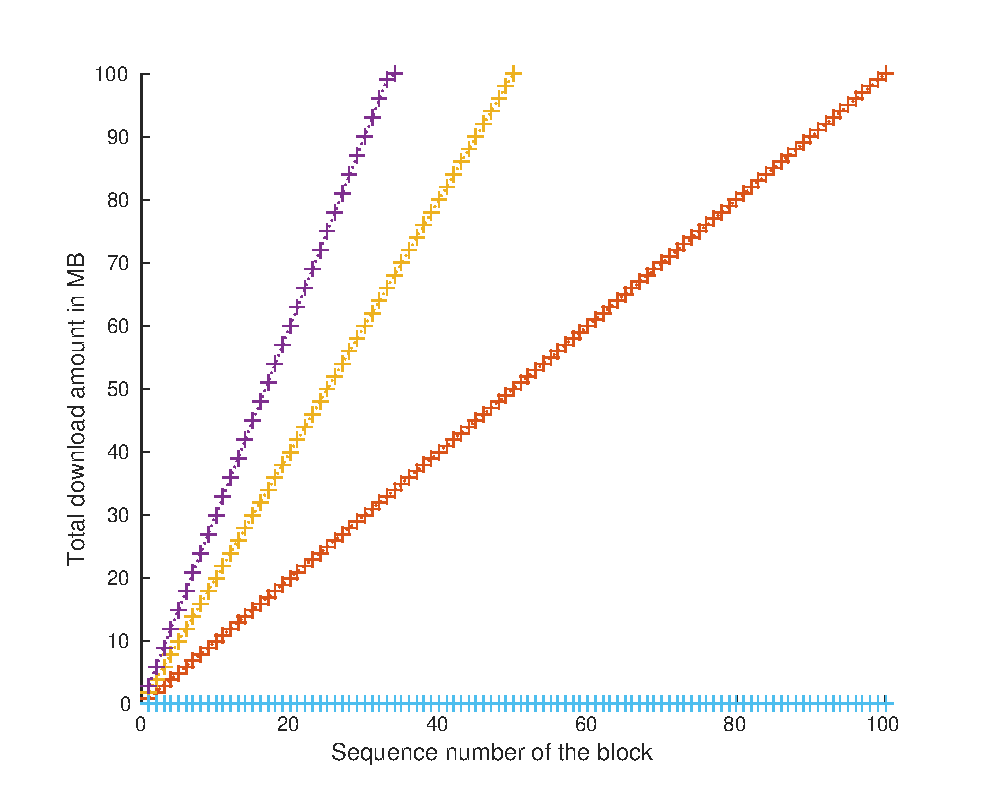
\includegraphics[scale=0.5]{experimentation/synthetic/synthetic-down.eps}}
\label{fig:synthetic-down}
}
\subfigure[Total upload amount.]{
\centerline{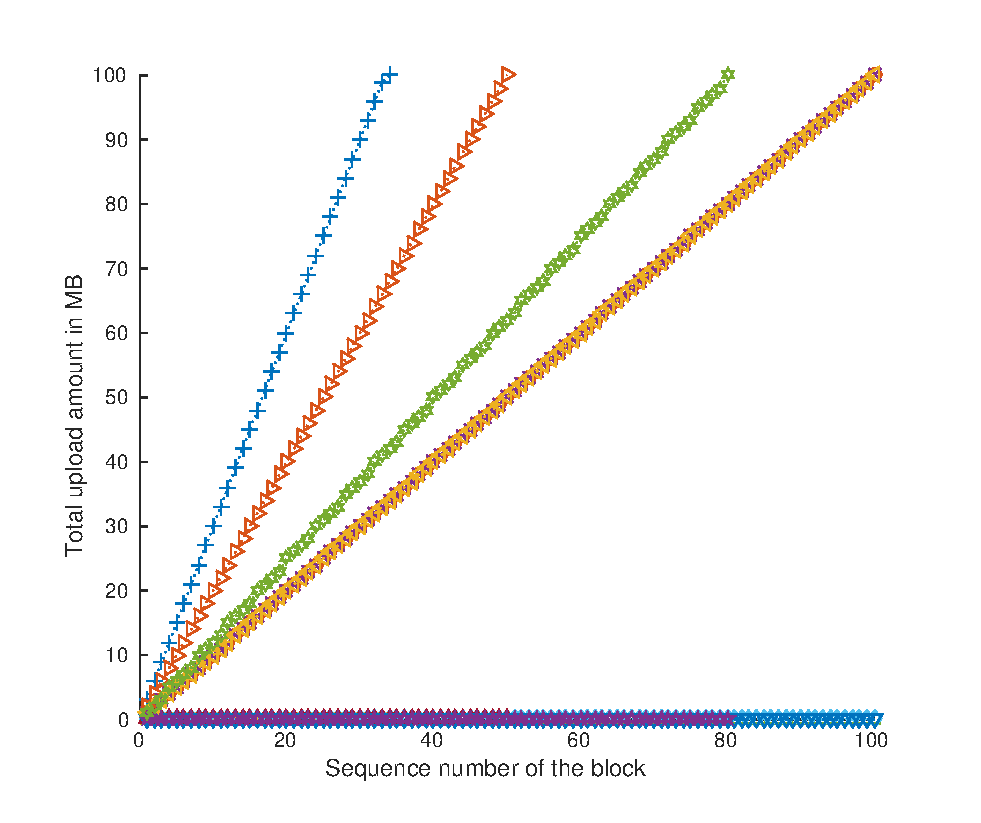
\includegraphics[scale=0.5]{experimentation/synthetic/synthetic-up.eps}}
\label{fig:synthetic-up}
}
\caption{Download and upload amounts during the experiment.}
\label{fig:synthetic-amounts}
\end{figure}

The total download and upload amounts of every peer is plotted in Figure \ref{fig:synthetic-amounts}.
Every datapoint is the total download amount in a block.
These datapoints are connected by a dotted line representing the link between these datapoints.
The plots show that MultiChain is able to correctly track the download and upload amounts without a problem.
There are no hitches in the figures and the amounts go up in fixed increments corresponding to the different speeds.
This means that MultiChain is fast enough to correctly track the amounts.

The download speeds below the threshold of 1000 MB of the scheduler
are not distinguishable from the download at the threshold speed.
This is because the scheduler waits until the threshold is reached before initiating the block.
The amount is tracked in the same amount of blocks,
but the total time of the experiment is longer for these experiments.
If the speed goes above the threshold, then this is reflected in the figure.

The graph in Figure \ref{fig:synthetic-graph} shows the MultiChain created by the experiment.
The graph is disconnected, because the different pairs of seeders and leechers did not interact with each other.
So no block that would connect their chains is created,
This leaves the graph disconnected.

\begin{figure}
	\centerline{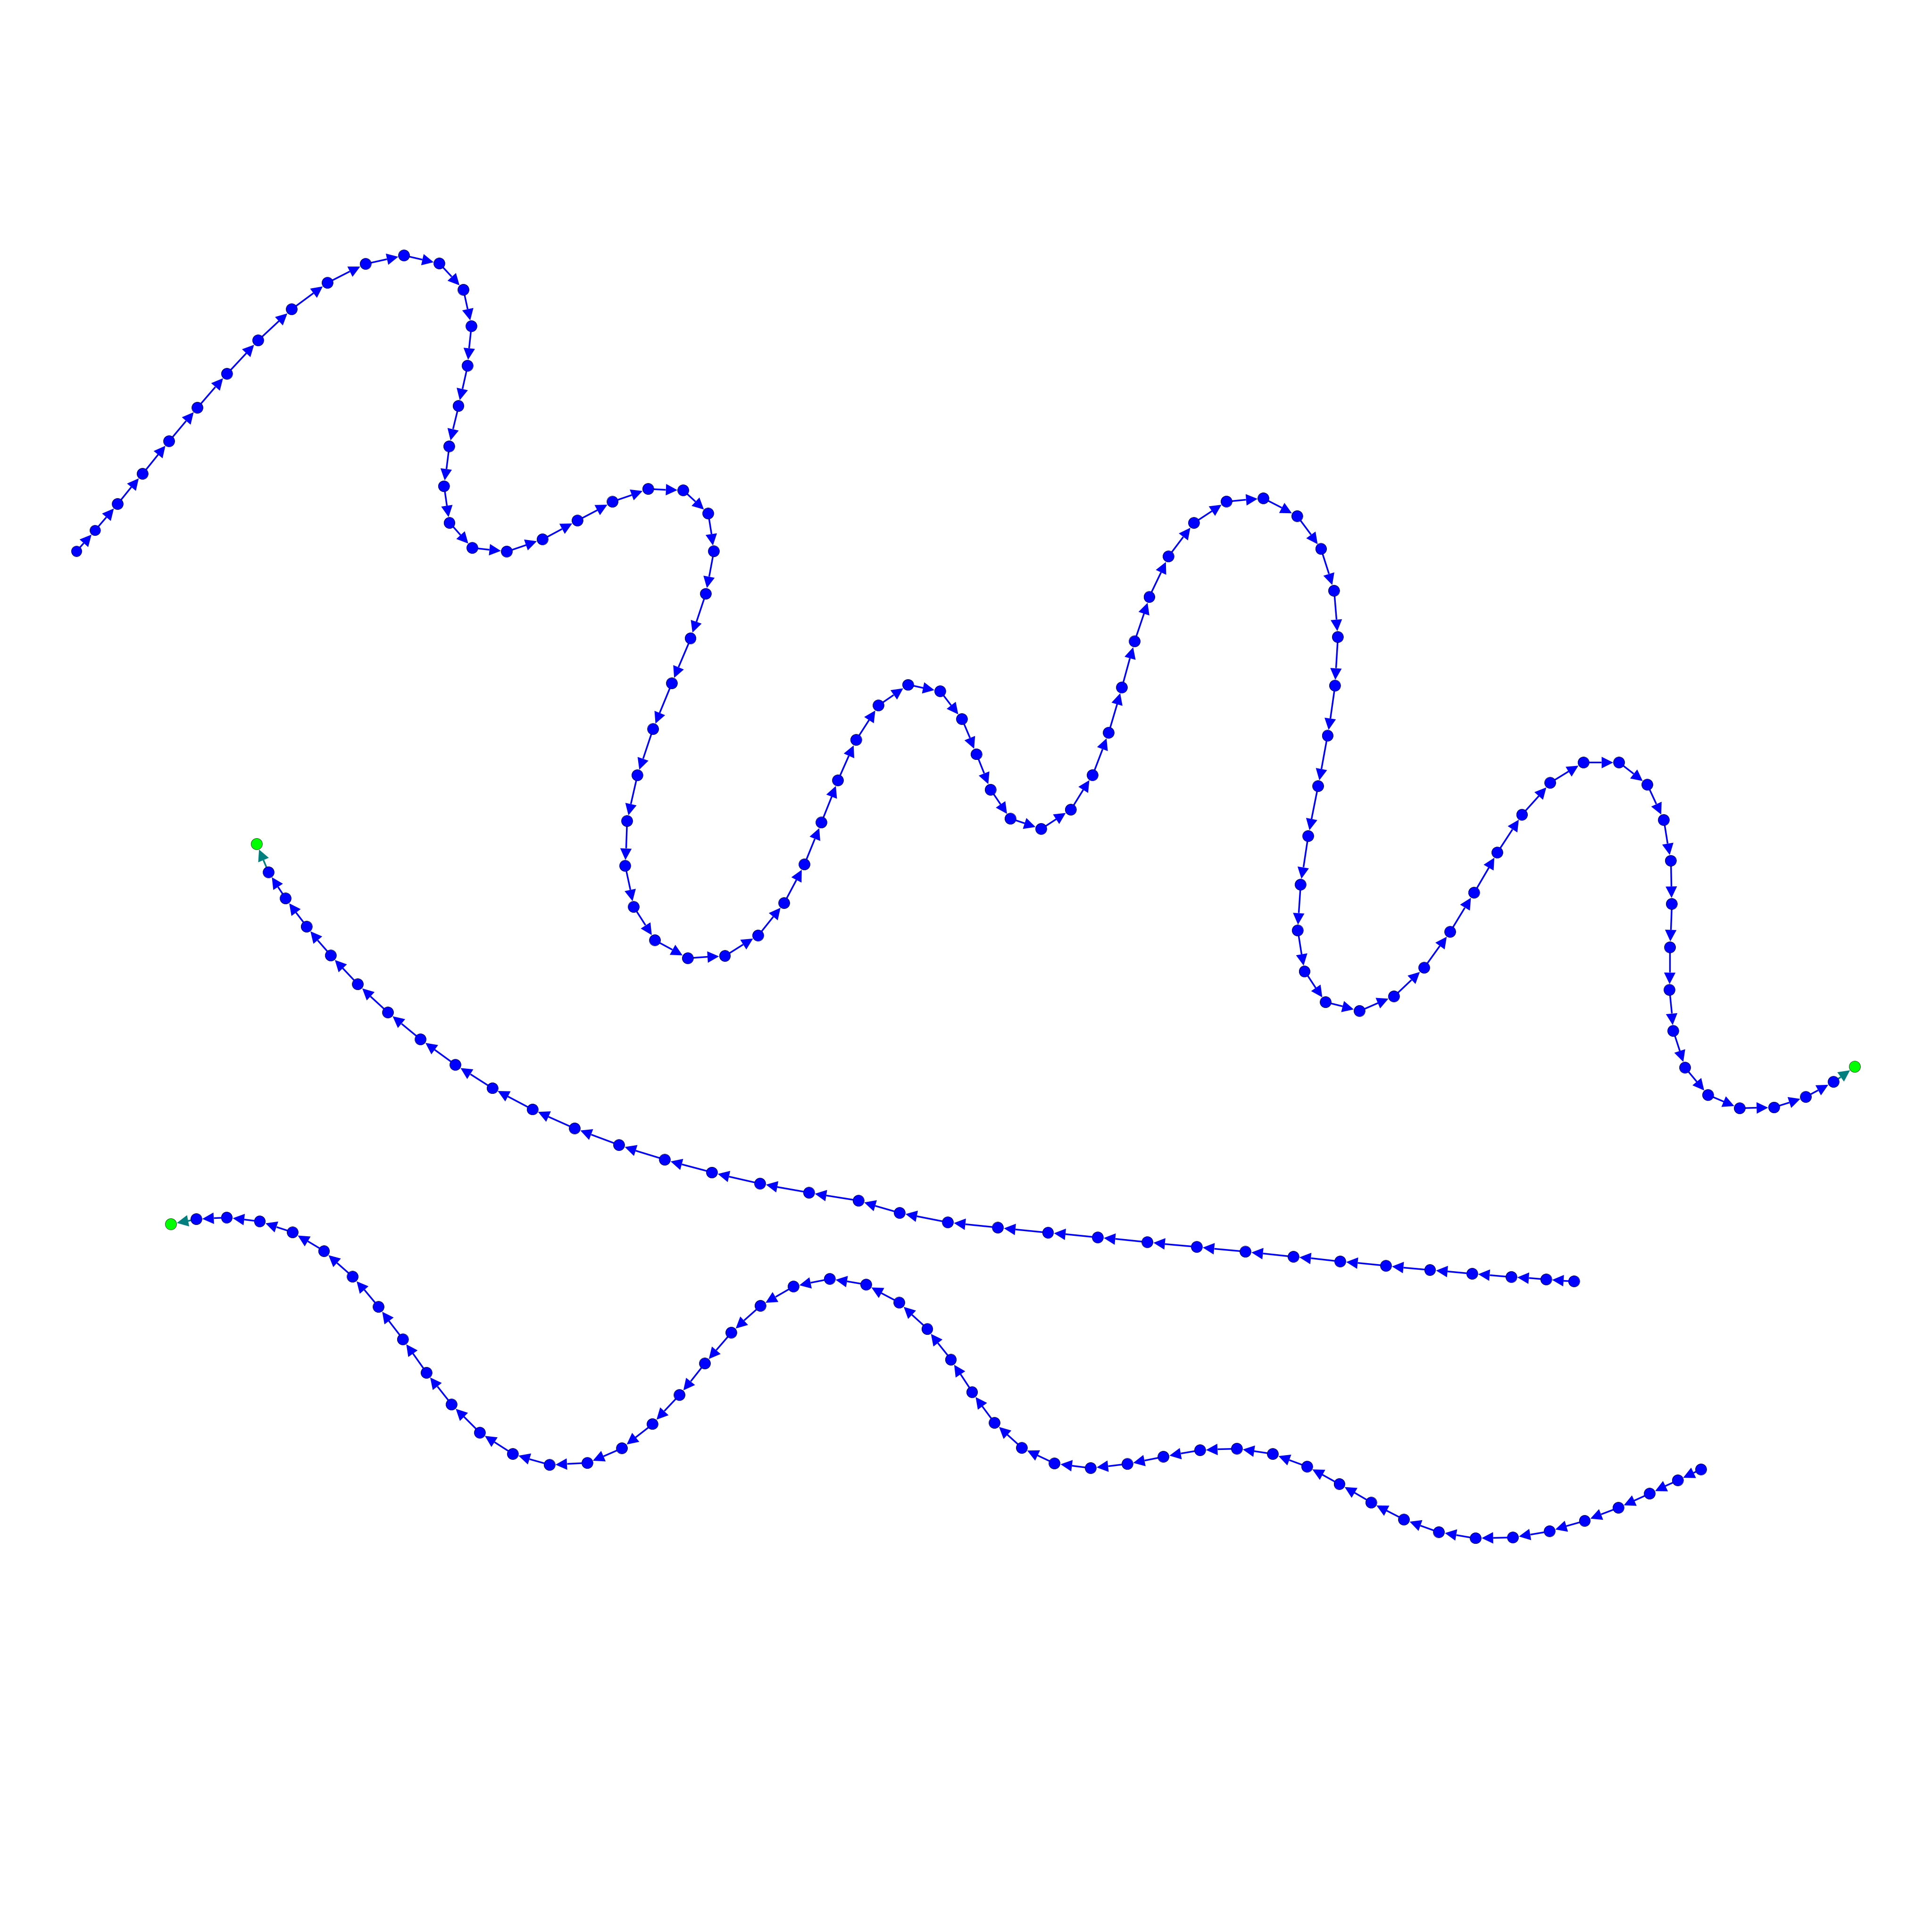
\includegraphics[scale=0.06]{experimentation/synthetic/synthetic.png}}
	\caption{Capturing a download in MultiChain.}
	\label{fig:synthetic-graph}
\end{figure}

This experiment was run several times before the final version in this report was run.
Earlier versions of the experiment resulted in two bugfix and two improvements:
the ability of the scheduler to create a block at the end of a download.
The experiment was also run multiple times because Dispersy does not always connect to every peer.
At the start of the experiment the peers are forced to be introduced,
but this does not always succeed.
This is a problem in discoverability and has been experienced by previous work aswell\cite{ruigrok-anonymous}.
This also happens when downloading a torrent in the real world.
The final version is chosen when Dispersy did connect all the peers.

\subsubsection{Anonymous download}
In an anonymous download scenario the data is downloaded through multiple hops.
The data is passed through the hops.
In the following experiment we mimick this scenario.
Data passes through multiple hops before it reaches the endpoint.




\section{Drop event recovery}
\label{sect:deadlock-exp}
MultiChain can run during normal operation into a situation
where a multiple of peers request to create blocks from each other as explained in section \ref{sect:deadlock}.
A specific experiment was conducted that created the situation manually.
This situation was also encountered during experimentation
and the experiment shows MultiChain correctly recovering from this situation.

\subsection{Forced drop event}
In this experiment a MultiChain node 1 tries to send a request to node 2 to create a block.
Node 2 is specifically configured for the purpose of the experiment
to ignore and drop all requests.
Node 1 now should wait for the response of the other node for a specific time.
During the time that node 1 is waiting a different request is sent from a normal node 3 to node 1.
This request will be dropped by node 1,
as it cannot process any incoming requests while node 1 has an outstanding request.
Node 1 and node 2 should timeout and continue operations.
After that node 2 will retransmit a request to node 1 and this should be completed correctly.

The experiment is locally run using gumby with all nodes running on a single computer.
Only three instances of MultiChain communities are started.
One of these instances never respond to a request to construct a block.
The logging of the every node is captured and recorded to verify the results of the experiment.

The output of the logging can be seen in Figure \ref{fig:manual-deadlock-experiment}.
First node 1 sends a signature request to node 2.
This message is ignored by node 2.
During the waiting period of node 1 a block request is sent to node 1 by node 3.
This request is also ignored, because node 1 cannot perform operations on the chain.
After the timeout period both node 1 and node 2 save an half-signed block to their chain
and can continue operations.
This is validated by a block created between node 3 and node 1.

\begin{figure}
\begin{FVerbatim}[fontsize=\small]
1: Requesting Signature for candidate: 2
1: Chain Exclusion: signature request: False
1: Chain Exclusion: acquired, sending signature request.
1: Sending signature request.
2: Received signature request that will be ignored.

3: Requesting Signature for candidate: 1
3: Chain Exclusion: signature request: False
3: Chain Exclusion: acquired, sending signature request.
3: Sending signature request.
1: Received signature request.
1: Chain Exclusion: process request: True
1: Chain Exclusion: not acquired. Dropping request.

1: Timeout received for signature request.
1: Persisting sr: bFOXhHT2ffSrtIn9tuMfEGGarGY=
3: Timeout received for signature request.
3: Persisting sr: l1O8UquXdxWdkg+KAYZ1FYocwjo=
3: Requesting Signature for candidate: 1

3: Chain Exclusion: signature request: False
3: Chain Exclusion: acquired, sending signature request.
3: Sending signature request.
1: Received signature request.
1: Chain Exclusion: process request: False
1: Chain Exclusion: acquired to process request.
1: Persisting sr: 7Y86Ck4duwTduP6j/aIRrWHAZqw=
1: Sending signature response.
3: Signature response received. Modified: True
3: Valid 1 signature response(s) received.
3: Persisting sr: 7Y86Ck4duwTduP6j/aIRrWHAZqw=
3: Chain exclusion: released received signature response.
\end{FVerbatim}
    \caption{Output of the manual drop event experiment}~\label{fig:manual-deadlock-experiment}
\end{figure}

\subsection{Naturally occuring drop events}
In the experiment a 100 megabyte file was downloaded anonymously with 2 hops.
Anonymously downloading is described more in the thesis report of R. Ruigrok~\cite{ruigrok-anonymous}.
There are 2 Triblers instances with exit functionality and 18 instances without exit functionality.
All instances are run locally on one machine.
The instances are run in parallel,
so the fact that all instances are run on a single machine does not cause the drop event to occur.
There is no packetloss in this experiment.
The corresponding graph of all the MultiChains of the experiment can be seen in Figure \ref{fig:deadlock-double}.

The potential scenario of two peers both waiting can be seen multiple times in the graph and are encircled.
The scenario generates a half-signed block at both peers.
Usually the peers continue collaboration and this continuation of a sequence can be seen in subsequent blocks.
In the graph a more complicated scenario can also be seen where multiple peers timeout between each other.
The graph shows that MultiChain correctly recovers from all scenario's.

\begin{figure}
	\centerline{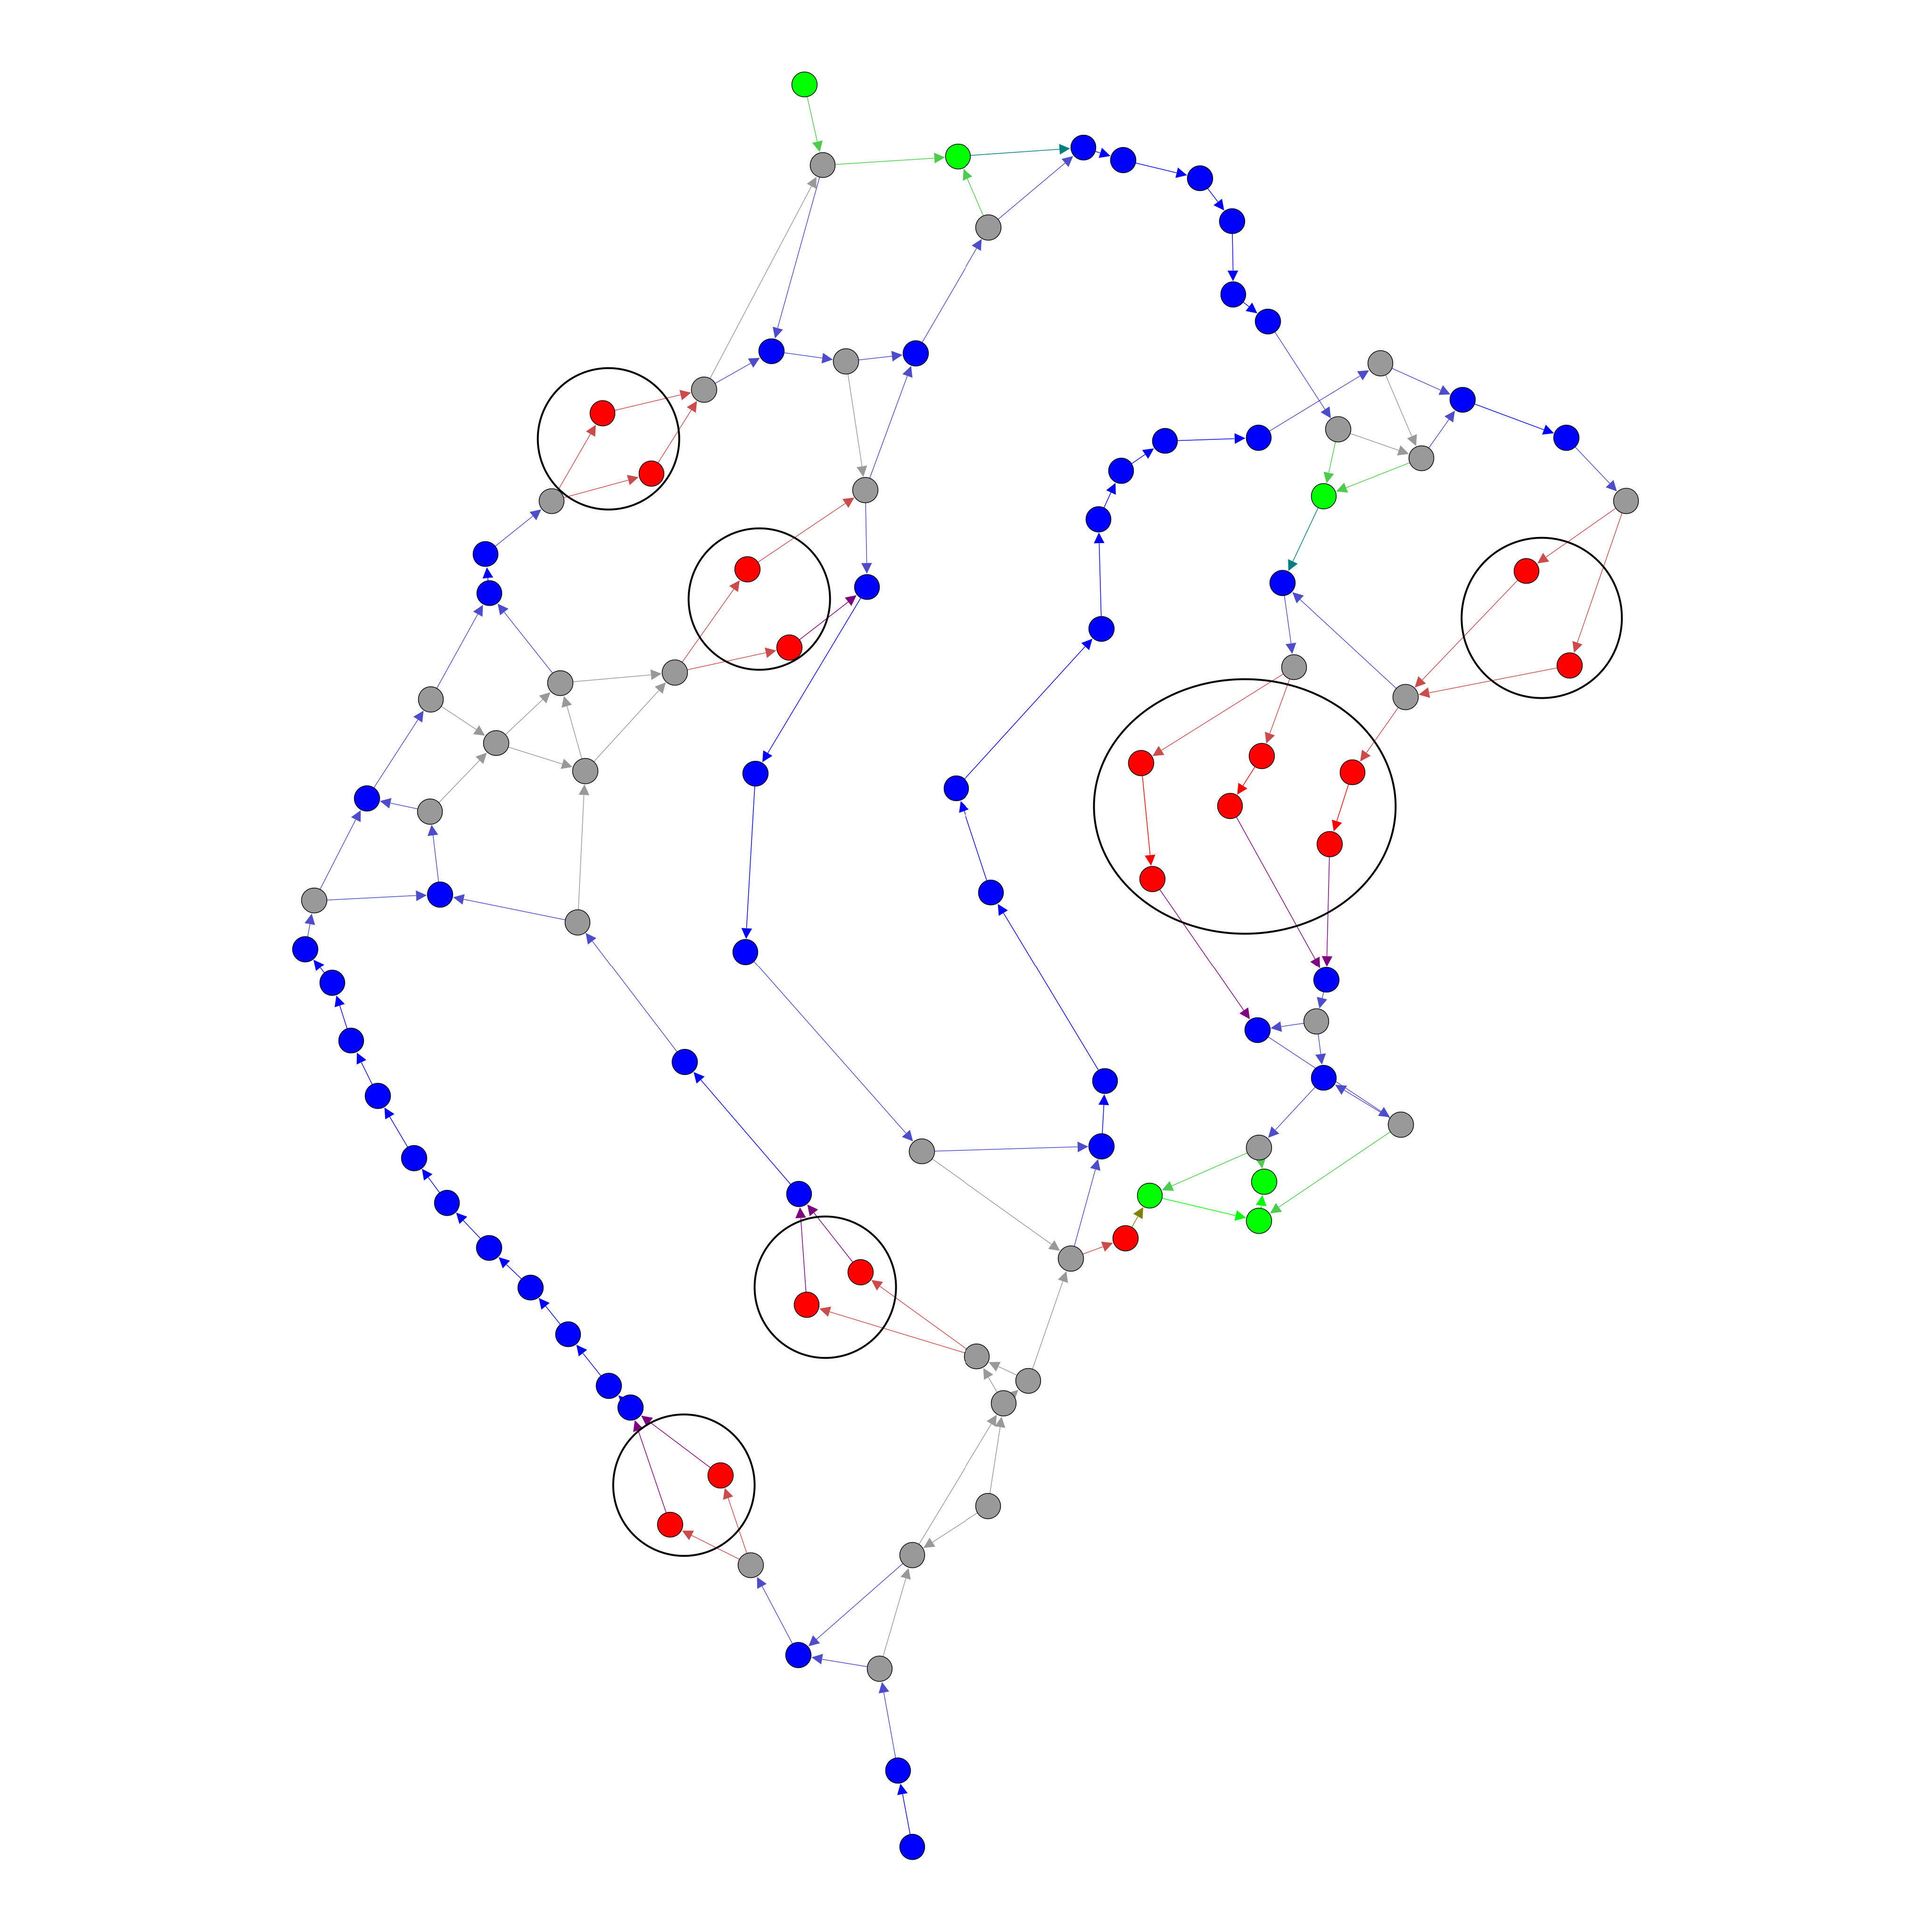
\includegraphics[scale=0.1]{experimentation/deadlock/deadlock.png}}
	\caption{Mixing of double-signed blocks(blue/grey) and half-signed blocks(red) in MultiChain.}
	\label{fig:deadlock-double}
\end{figure}

